\documentclass[11pt,a4paper]{article}

\usepackage[margin=1in, paperwidth=8.3in, paperheight=11.7in]{geometry}
\usepackage{amsmath,amsfonts,fancyhdr,bbm,graphicx,tikz}
\usetikzlibrary{automata,positioning}
\graphicspath{ {img/} }
\usepackage[section,nohyphen]{DomH}
\headertitle{Stochastic Optimisation - Notes}

\begin{document}

\title{Stochastic Optimisation - Notes}
\author{Dom Hutchinson}
\date{\today}
\maketitle

\tableofcontents\newpage

\section{Multi-Armed Bandit}

\subsection{The Problem}

\begin{example}{Motivating Example}
  Consider having a group of patients and several treatments they could be assigned to. How best do you go about determining which treatment is best? The obvious approach is to assign some of the patients randomly and then assign the rest to the best treatment, but how much evidence is sufficient? And how likely are you to choose a sub-optimal treatment?
\end{example}

\begin{definition}{Multi-Armed Bandit Problem}
   An agent is faced with a choice of $K$ actions. Each (discrete) time step the agent plays action $i$ they receive a reward from the random real-valued distribution $\nu_i$. Each reward is independent of the past. The distributions $\nu_1,\dots,\nu_K$ are unknown to the agent.\\
   In the \textit{Multi-Armed Bandit Problem} the agent seeks to maximise a measure of long-run reward.
\end{definition}

\begin{remark}{Informal Definition of Multi-Armed Bandit Problem}
  Given a finite set of actions and a random reward for each action, how best do we learn the reward distribution and maximise reward in the long-run.
\end{remark}

\begin{definition}{Formal Definition of Multi-Armed Bandit Problem}
  Consider a sequence of (unknown) mutually independent random variables $\{X_i(t)\}_{i\in[1,K]}$, with $t\in\nats$. Consider $X_i(t)$ to be the distribution of rewards an agent would receive if they performed action $i$ at time $t$. Since the rewards are independent of the past $X_i(t),X_i(t+1),\dots$ are IID random variables. The \textit{Multi-Armed Bandit Problem} tasks us to find the greatest expected reward from all the actions.
  \[ \mu^*:=\max_{i=1}^K\mu_i\quad\text{where }\mu_i=\expect(X_i(t)) \]
  There are a number of ways to formalise this objective.
\end{definition}

\begin{remark}{Assumptions}
  For the \textit{Multi-Armed Bandit Problem} we make the following assumptions about the set up
  \begin{itemize}
    \item When action $i$ is played only the realisation of $X_i(t)$ is observed and none of $X_j(t),\ j\neq i$, are observed. Thus when the agent's $t^{th}$ action is played only the rewards of actions $\{1,\dots,t-1\}$ are known to the agent.
    \item The agent has access to an external source of randomness which is used to choose it's next action.
  \end{itemize}
\end{remark}

\begin{definition}{Strategy, $I(\cdot)$}
  Our agent's strategy $I:\nats\to[1,K]$ is a function which determines which action the agent shall make at a given point in time. The strategy can use the knowledge gained from previous actions \& their rewards only.
  \[ I(t)=I\big(t,\underbrace{\{I(s)\}_{\in[1,t)}}_\text{Prev. Actions},\underbrace{\{X_{I(s)}(s)\}_{\in[1,t)}}_\text{Prev. Rewards}\big)\in[1,K] \]
\end{definition}

\begin{definition}{Long-Run Average Reward Criterion, $X_*$}
  For a strategy $I(\cdot)$ we define the following measure for \textit{Long-Run Average Reward}
  \[ {\displaystyle X_*=\lim_{T\to\infty}\inf\frac1T\sum_{t=1}^T\expect(X_{I(t)})} \]
  The \textit{Infinum} is taken as there is no guarantee the limit exists (depending on the strategy), typically we will only deal with strategies where this limit exists.\\
  Most strategies as based only on realisations of $\{X_i(s)\}_{s\in[1,t)}$, thus $\expect(X_{I(t)})\leq\mu^*$ and thus $X_*\leq\mu^*$. A strategy $I(\cdot)$ is \textit{Optimal} if $X_*=\mu^*$.
\end{definition}

\begin{remark}{It is not hard to find an \textit{Optimal Strategy} in the (very) long run, so we are going to look at \textit{Regret Minimisation First}.}
\end{remark}

\subsection{Regret Minimisation}

\begin{definition}{Regret, $R_n$}
  \textit{Regret} is a measure of how much reward was lost during the first $n$ time steps. The \textit{Regret} $R_n$ of a strategy $\{I(t)\}_{t\in\nats}$ in the first $n$ time steps is given by
  \[\begin{array}{rcl}
    R_n&=&{\displaystyle \max\limits_{k=1}^K\sum_{t=1}^n \expect[\underbrace{X_k(t)}_\text{Best Pos}-\underbrace{X_{I(t)}(t)}_\text{Actual}]}\\
    &=&n\mu^*-{\displaystyle\sum_{t=1}^n\expect\big[X_{I(t)}(t)\big]}
  \end{array}\]
  \textit{Regret} only involves expectation and thus can be learnt from observations. We want to produce a strategy where \textit{Total Regret} grows sub-linearly.(i.e. $R_T/T\overset{T\to\infty}\longrightarrow0$)
\end{definition}

\begin{remark}{Minimising the growth rate of $R_T$ with $T$ is quite hard.}
  The best achievable regret scales as $R_T\sim c\log T$ (i.e. $R_T/c\log T\overset{T\to\infty}\longrightarrow1$) where $c$ depends on the reward distributions $X_1(t),\dots,X_K(t)$.
\end{remark}

\begin{definition}{Pseudo-Regret, $\tilde{R}_n$}
  \textit{Pseudo-Regret} $\tilde{R}_n$ is a less popular alternative to \textit{Regret} $R_n$.
  The \textit{Pseudo-Regret} $R_n$ of a strategy $\{I(t)\}_{t\in\nats}$ in the first $n$ time steps is given by
  \[ \tilde{R}_n=\max\limits_{k=1}^K\sum_{t=1}^n\big(X_k(t)-X_{I(t)}(t)\big) \]
  \textit{Pseudo-Regret} includes intrinsic randomness (which is independent of the past) and thus cannot be learnt from observations.
\end{definition}

\subsection{Best Arm Identification for Bernoulli Distribution}

\begin{example}{Best Arm Identification for Bernoulli Bandits}
  Consider a bandit with two \textit{Bernoulli} arms: $\{X_1(t)\}_{t\in\nats}$ IID RVs with distribution $\text{Bern}(\mu_1)$; and, $\{X_2(t)\}_{t\in\nats}$ IID RVs with distribution $\text{Bern}(\mu_2)$. \\
  Suppose $\mu_1>\mu_2$ (i.e. arm 1 is better). Let the player play each arm $n$ times and declare the arm with the greatest empirical mean to be the better arm. \textit{What is the probability of choosing the wrong arm (Arm 2)?}.\\
  \\
  An error occurs if $\sum_{t=1}^nX_2(t)\geq\sum_{t=1}^nX_1(t)$ and thus we want to calculate the probability of this event.\\
  Define $\{Y(t)\}_{t\in\nats}$ st $Y(t):=\{X_2(t)-X_1(t)$. This means $Y(t)\in\{-1,0,1\}\subset[-1,1]$.\\
  To use \textit{Hoeffding's inequality} we need to scale $Y$ to be in $[0,1]$, so we define $Z(t):=\frac12(Y(t)+1)$. We have $\expect(Z(t))=\frac12(1+\mu_2-\mu_1)$ and an error occurs if $\sum_{t=1}^nY(t)>0\Longleftrightarrow \sum_{t=1}^nZ(t)\geq\frac{n}2$. By \textit{Hoeffding's Inequality}
  \[\begin{array}{rclll}
    \prob(\text{error})&=&\displaystyle\prob\left(\sum_{i=1}^nZ(t)\geq\frac{n}2\right)\\
    &=&{\displaystyle\prob\left(\left(\sum_{i=1}^nZ(t)\right)-\frac{n}2(1+\mu_2-\mu_1)\geq\frac{n}2(\mu_1-\mu_2)\right)}\quad\text{subtracting $\mu$ from both sides}\\
    &=&{\displaystyle\prob\left(\sum_{i=1}^n\bigg(X_i-\underbrace{\frac{1}{2}(1+\mu_2-\mu_1)}_\mu\bigg)\geq n\underbrace{\frac12(\mu_1-\mu_2)}_t\right)}\quad\text{arranging for Hoeffding's}\\
    &\leq&\exp\left(-2n\cdot\frac{1}4(\mu_1-\mu_2)^2\right)\quad\text{by Hoeffding's Inequality}\\
    &=&\exp\left(-\frac{n}2(\mu_1-\mu_2)^2\right)
  \end{array}\]
\end{example}

\subsection{Heuristic}

\section{Probability}

\begin{definition}{Random Process}
  A \textit{Random Process} is a collection of random variables indexed by time $\{X_t\}_{t\in T}$ (e.g. flipping a coin several times). Each of these random variables can take a value from a state space $S$. A random process a \textit{Discrete Time Process} if the index set $T$ is discrete. A random process a \textit{Continuous Time Process} if the index set $T$ is continuous.
\end{definition}

\subsection{Probability Inequalities}

\begin{remark}{We can use the moments of a random variable to determine bounds on the probability of it taking values in a certain set.}
\end{remark}

\begin{theorem}{Markov's Inequality}
  Let $X$ be a non-negative random variable. Then
  \[ \forall\ c>0\quad\prob(X\geq c)\leq\frac{\expect(X)}c \]
  \textit{Proof}\\
  Consider an event $A$ and define its indicator $\mathbbm{1}(A)(\omega):=\begin{cases}1&\omega\in A\\0&\omega\not\in A\end{cases}$. Fix $c>0$, then
  \[\begin{array}{rrcl}
    &\expect(X)&\geq&\expect[X\mathbbm{1}(X\geq c)]\\
    &&\geq&\expect[c\mathbbm1(X\geq c)]\\
    &&=&c\prob(X\geq c)\\
    \implies&\prob(X\geq c)&\leq&\frac1c\expect(X)
  \end{array}\]
\end{theorem}

\begin{theorem}{Chebyshev's Inequality}
  Let $X$ be a random-variable with finite mean and variance. Then
  \[ \forall\ c>0\quad\prob(|X-\expect(X)|\geq c)\leq\frac{\var(X)}{c^2}\]
  \textit{Proof}\\
  Note that the events $|X-\expect(X)|\geq c$ and $(X-\expect(X))^2\ge c^2)$ are equivalent. Note that $\var([X-\expect(X)]^2)=\var(X)$. Then the result follows by \textit{Markov's Inequality}.
\end{theorem}

\begin{theorem}{Chebyshev's Inequality for Sum of IIDs}
  Let $X_1,\dots,X_n$ be IID random variables with finite mean $\mu$ and finite variance $\sigma^2$.
  \[ \forall\ c>0\quad\prob\left(\left|\left(\sum_{i=1}^nX_i\right)-n\mu\right|\geq nc\right)\leq\frac{\sigma^2}{nc^2} \]
  \textit{Proof}\\
  This is proved by extending the proof of \texttt{Theorem 2.2} and noting that the variance of a sum of IIDs is the sum of the individual variances.
\end{theorem}

\begin{theorem}{Chernoff Bounds}
  Let $X$ be a random variable whose moment-generating function $\expect[e^{\theta X}]$ is finite $\forall\theta$. Then
  \[ \forall\ c\in\reals\quad\prob(X\geq c)\leq\inf_{\theta>0}e^{-\theta c}\expect(e^{\theta X})\quad\text{and}\quad\prob(X\leq c)\leq\inf_{\theta<0}e^{-\theta c}\expect(e^{\theta X}) \]
  \textit{Proof}\\
  Note that the events $X\geq c$ and $e^{\theta X}\geq e^{\theta c}$ are equivalent for all $\theta>0$. The result follows by applying \textit{Markov's Inequality} to $r^{\theta X}$ and taking the best bound over all possible $\theta$.
  \[\begin{array}{rcl}
    \prob(X\geq c)&=&\prob(e^{\theta X}\geq e^{\theta c})\\
    &\leq&e^{-\theta c}\expect(e^{\theta X})\\
    &\leq&\inf_{\theta<0}e^{-\theta c}\expect(e^{\theta X}) %TODO check this step
  \end{array}\]
\end{theorem}

\begin{theorem}{Chernoff Bounds for Sum of IIDs}
  Let $X_1,\dots,X_n$ be IID random variables. Then $\forall\ c\in\reals$
  \[\begin{array}{rcl}
    {\displaystyle\prob\left(\sum_{i=1}^nX_i\geq nc\right)}&\leq\inf\limits_{\theta>0}e^{-n\theta c}\left(\expect\left[e^{\theta X}\right]\right)^n\\
    {\displaystyle\prob\left(\sum_{i=1}^nX_i\leq nc\right)}&\leq\inf\limits_{\theta<0}e^{-n\theta c}\left(\expect\left[e^{\theta X}\right]\right)^n
  \end{array}\]
\end{theorem}

\begin{theorem}{Jensen's Inequality}
  Let $f$ be a \textit{Convex Function} and $X$ be a random variable. Then
  \[ \expect[f(X)]\geq f(\expect[X]) \]
\end{theorem}

\begin{theorem}{Bound on Moment Generating Function}
  Let $X$ be a random variable taking values in $[0,1]$ with finite expected value $\mu$. Then we can bound the MGF of the centred random variable with
  \[ \forall\ \theta\in\reals\quad\expect\left[e^{\theta(X-\mu)}\right]\leq e^{\theta^2/8} \]
  \textit{Proof (of weaker version)}\\
  Let $X_1$ be an independent copy of $X$, so both have mean $\mu$. We can easily verify that $f(x)=e^{\theta x}$ is a convex function for all $\theta\in\reals$. By \textit{Jensen's Inequality} to $f(\cdot)$ and $X_1$
  \[ \expect[e^{-\theta X_1}]\geq e^{-\theta\expect[X_1]}=e^{-\theta\mu}\quad(1) \]
  Consequently
  \[\begin{array}{rrclll}
  &\expect[e^{\theta(X-X_1)}]&=&\expect[e^{\theta X}]\cdot\expect[e^{-\theta X_1}]&\quad&\text{by independence}\\
  &&\geq&\expect[e^{\theta X}]\cdot e^{-\theta\mu}&&\text{by (1)}\\
  &&=&\expect[e^{\theta(X-\mu)}]\\
  \implies&\expect[e^{\theta(X-X_1)}]&\geq&\expect[e^{\theta(X-\mu)}]
  \end{array}\]
  Since $X,X_1\in[0,1]$ then $(X-X_1)\in[-1,1]$. As $X,X_1$ have the same distribution $\expect(X-X_1)=0$ and the distribution is symmetric around the mean.\\
  Define random variable $S$ which is independent of $X,X_1$ and takes values $\{-1,1\}$, each with probability $p=\frac12$. $S(X-X_1)$ has the same distribution as $(X-X_1)$ due to independence of $S$ and symmetry of $(X-X_1)$. Hence
  \[\begin{array}{rclll}
    \expect[e^{\theta(X-X_1)}]&=&\expect[e^{\theta S(X-X_1)}]&\quad&\text{by identical distribution}\\
    &\leq&\expect[e^{\theta S}]&&(2)\text{ since }(X-X_1)\in[-1,1]\\
    &=&\frac12(e^\theta+e^{-\theta})&&\text{ by def. of expectation}\\
    \implies\expect[e^{\theta(X-X_1)}]&\leq&\frac12(e^\theta+e^{-\theta})
  \end{array}\]
  Note that $f(x)=e^x+e^{-x}$ is increasing for $x\in(0,\infty)$; decreasing for $x\in(-\infty,0)$; and symmetric around $0$.\\
  Using a \textit{Taylor Series} we an observed that
  \[\begin{array}{rclll}
  \frac12(e^\theta-e^{-\theta})&=&{\displaystyle\sum_{n=0}^\infty}\frac{\theta^{2n}}{(2n)!}&\quad&\text{by Taylor expansion of}e^x\\
  &\leq&\displaystyle\sum_{n=0}^\infty\frac{(\theta^2/2)^n}{n!}\\
  &\overset{\text{def.}}{=}&e^{\theta^2/2}\\
  \implies\frac12(e^\theta+e^{-\theta})&\leq&e^{\theta^2/2}
  \end{array}\]
  Combining all these results we get
  \[ \begin{array}{rl}
  &\expect[e^{\theta(X-\mu)}]\leq\expect[e^{\theta(X-X_1)}]\leq\frac12(e^\theta+e^{-\theta})\leq e^{\theta^2/2}\\
  \implies&\expect[e^{\theta(X-\mu)}]\leq e^{\theta^2/2}
  \end{array}\]
  \proved
\end{theorem}

\begin{theorem}{Hoeffding's Theorem}
  Let $X_1,\dots,X_n$ be IID random variables taking values in $[0,1]$ and with finite expected value $\mu$. Then
  \[ \forall\ t>0\quad\prob\left(\sum_{i=1}^n(X_i-\mu)>nt\right)\leq e^{-2nt^2} \]
  \textit{Proof}\\
  From \textit{Chernoff's Bound} we have that
  \[ \forall\ \theta>0\quad\prob\left(\sum_{i=1}^n(X_i-\mu)>nt\right)\leq e^{-\theta nt}\left(\expect[e^{\theta(X-\mu)}]\right)^n \]
  Using \texttt{Theorem 2.7} to bound the moment generating function, we get
  \[ \forall\ \theta>0\quad\prob\left(\sum_{i=1}^n(X_i-\mu)>nt\right)\leq e^{-\theta nt}\cdot e^{n\frac{\theta^2}8}=e^{n\left(-\theta t+\frac{1}8\theta^2\right)} \]
  Thus, by taking $\log$s and rearranging, we get
  \[ \forall\ \theta>0\quad\frac1n\log\prob\left(\sum_{i=1}^n(X_i-\mu)>nt\right)\leq-\theta t+\frac{\theta^2}8 \]
  We have that $-\theta t+\frac{\theta^2}8$ is minimised at $\theta=4t$ which is positive if $t$ is positive. Thus, by applying this bound and substituting $\theta=4t$ we get
  \[ \forall\ \theta>0\quad\prob\left(\sum_{i=1}^n(X_i-\mu)>nt\right)\leq e^{n\left(-4t^2+\frac{1}8(16t^2)\right)}=e^{n(-4t^2+2t^2)}=e^{-2nt^2} \]
  \proved
\end{theorem}

\subsection{Markov Chains}

\begin{definition}{Markov Property}
  A random process has the \textit{Markov Property} if the conditional probability of a future state \underline{only} depends on the current state.
  \[ \prob(X_{t+1}=y|X_{t}=x_t,X_{t-1}=x_{t-1})=\prob(X_{t+1}=y|X_t=x_t) \]
  A random process with the \textit{Markov Property} is called a \textit{Markov Process/Chain}.
\end{definition}

\begin{remark}{On this course we only deal with discrete time markov chains}\end{remark}

\begin{proposition}{Characterising a Markov Process}
  A \textit{Markov Process} can be characterised by the set of all $1$-step conditional probabilities
  \[ \prob(X_{t+1}=y|X_t=x)\ \forall\ x,y\in S \]
  A markov chain is \textit{time-homogeneous} if the $1$-step conditionals only depend on $x,y$ and not on $t$ ($\prob(X_{t+1}=y|X_t=x)=\prob(X_1=t|X_0=x)$). The $1$-step conditional probabilities of a \textit{time-homogeneous markov process} can be specified in an $|S|\times |S|$ matrix $P$ where
  \[ p_{x,y}=\prob(X_{t+1}=y|X_t=x) \]
  $P$ is a \textit{Stochastic Matrix}.
\end{proposition}

\begin{proposition}{$n$-Step Transition Probabilities from $1$-Step Transition Matrix}
  Let $P$ be the $1$-step transition matrix for a \textit{time-homogeneous}.

  \par The $2$-step transition probabilities (ie $\prob(X_{t+2}=z|X_t=x)$) can be found as
  \[\begin{array}{rcll}
    \prob(X_{t+2}=z|X_t=x)&=&\prob(X_2=z|X_0=x)&\text{by time-homogeneity}\\
    &=&\sum_{y\in S}\prob(X_2=z,X_1=y|X_t=x)\\
    &=&\sum_{y\in S}\prob(X_1=y|X_0=x)\prob(X_2=z|X_1=t,X_0=x)\\
    &=&\sum_{y\in S}\prob(X_1=y|X_0=x)\prob(X_2=z|X_1=y)\\
    &=&\sum_{y\in S}p_{xy}p_{yz}\\
    &\equiv&[P^2]_{xz}
  \end{array}\]
  This can be generalise for the $n$-step transition probabilities with
  \[ \prob(X_{t+n}=z|X_t=x)=[P^n]_{xz} \]
\end{proposition}

\begin{proposition}{Any Joint Probability from $1$-Step Transition Matrix}
  For a time homogeneous markov process the joint distribution of any transition can be computed by considering the individual steps of the transition.
  \[ \prob(X_{n_0}=x_0,X_{n_1}=x_1,X_{n_2}=x_2,\dots)=\prob(X_{n_0}=x_0)\cdot[P^{n_0-n_1}]_{x_0x_1}\cdot[P^{n_1-n_2}]_{x_1x_2}\dots \]
\end{proposition}

\begin{proposition}{State Diagram Representation}
  A graph/automata can be drawn to represent the transition probability matrix $P$. A node is assigned for each member of the state space $S$ and an arrow is drawn between each pair of nodes $(x,y)$ where $P_{xy}\neq0$. Generally the value of $P_{xy}$ is denoted on the arrow.
  \begin{center}
    \[P=\begin{pmatrix}\frac{1}{2}&\frac{1}{2}&0\\\frac{1}{6}&\frac{1}{2}&\frac{1}{3}\\0&\frac{1}{2}&\frac{1}{2}\end{pmatrix}\]
    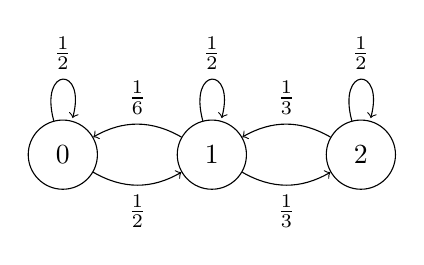
\begin{tikzpicture}
    	\node[state] (0) {0};
    	\node[state] (1)[right=of 0] {1};
    	\node[state] (2)[right=of 1] {2};

    	\path[->]
    	(0) edge [loop above] node {$\frac{1}{2}$} (0)
    	    edge [bend right] node[below] {$\frac{1}{2}$} (1)
    	(1) edge [loop above] node {$\frac{1}{2}$} (1)
    	    edge [bend right] node[above] {$\frac{1}{6}$} (0)
    	    edge [bend right] node[below] {$\frac{1}{3}$} (2)
    	(2) edge [loop above] node {$\frac{1}{2}$} (2)
    	    edge [bend right] node[above] {$\frac{1}{3}$} (1);
    \end{tikzpicture}
  \end{center}
\end{proposition}

\begin{definition}{Invariant Distribution}
  Let $\pmb\mu(t)$ denote the probability distribution of random variable $X$ (i,e, $\mu_x(t)=\prob(X_t=x)$). Then
  \[\begin{array}{rrcl}
    &\pmb\mu(t+1)&=&\prob(X_{t+1}=y)=\sum_{x\in S}\prob(X_t=x,X_{t+1}=y)=\sum_{x\in S}\mu_x(t)p_{xy}=\pmb\mu(t)P\\
    \implies&\pmb\mu(t+1)&=&\pmb\mu(t)P
  \end{array}\]
  A distribution $\pmb\pi$ on the state space is called an \textit{Invariant Distribution} if $\pmb\pi=\pmb\pi P$. If $X_t$ has distribution $\pmb\pi$ so will $X_{t+1},\dots$. Every markov chain with a \textit{finite} state space $S$ has an \textit{invariant distribution}. (Not necessarily true if $S$ is infinite).
\end{definition}

\begin{proposition}{Finding an Invariant Distribution}
  If an \textit{Invariant Distribution} it is easy to find by solving $\pmb\pi P=\pmb\pi$ and using normalising constant $\sum_{x\in S}\pi_x=1$.
\end{proposition}

\begin{definition}{Transience}
  A state $x\in S$ is \textit{Transient} if $\prob(\exists\ t>0: X_t=x|X_0=x)<1$. The number of times the markov chain returns to a transient state is finite, with probability 1.
\end{definition}

\begin{definition}{Recurrent}
  A state $x\in S$ is \textit{Recuurent} if $\prob(\exists\ t>0: X_t=x|X_0=x)=1$. The number of times the markov chain returns to a recurrent state is \underline{in}finite, with probability 1.
  \par Every markov chain, with a finite state space $S$, has a recurrent communicating class.
\end{definition}

\begin{definition}{Communication Class}
  We say $y\in S$ is \textit{Accessible} from $x\in S$ if $\exists\ t\geq0$ st $[P^t]_{xy}>0$.
  \par We say $x$ and $y$ \textit{communicate} (denoted $xCy$) if: $x$ is \textit{accessible} from $y$ and $y$ is \textit{accessible} from $x$.
  \par \textit{Communication} is an \textit{equivalence relation} on the state space $S$. Hence, \textit{communication} partitions $S$ into equivalence classes called \textit{Communication Classes}. All elements of a \textit{Communication Class} communicate with all other elements in the class, it is possible for elements to be accessible from another class but \underline{not} for those elements to \textit{communicate}.
  \par If one state in a \textit{Communicating Class} is \textit{Transient/Recurrent} then all states are in that class.
  \par If a \textit{Markov Chain} has only one communicating class it is called \textit{Irreducible}.
\end{definition}

\begin{remark}{If a Markov chain is irreducible, its invariant distribution (if one exists) is unique}
  If a \textit{Markov Chain} is irreducible and has a finite state space, then it has a unique invariant distribution.
\end{remark}

\begin{example}{Markov Chains}
  \begin{itemize}
    \item The \textit{Asymmetric Simple Random Walk} on $\ints$ is $\underbrace{\text{irreducible}}_\text{obvious},\ \underbrace{\text{transient}}_\text{not obvious}$ and has no invariant distribution.
    \item The \textit{Symmetric Simple Random Walk} on $\ints$ is $\underbrace{\text{irreducible}}_\text{obvious},\ \underbrace{\text{recurrent}}_\text{not obvious}$ and has no invariant distribution.
  \end{itemize}
\end{example}

\begin{theorem}{Ergodic Theorem for Markov Chains}
  Let $\{X_t\}_{t\in\nats}$ be an irreducible markov chain on state space $S$ (not necessarily finite) with unique invariant distribution $\pmb\pi$. Then
  \[ \forall\ x\in S\quad\lim_{t\to\infty}\frac1t\sum_{s=1}^t \indexed(X_s=x)=\pi_x\]
  i.e. The fraction of time spend in state $x\in S$ tends to $\pi_x$ in the long run.
\end{theorem}

\begin{definition}{Period}
  The \textit{Period} of a state $x\in S$ is the greatest common divisor of all possible return times to $x$
  \[ \text{Period}(x):=\text{gcd}\big(\{t>0:\prob(X_t=x|X_0=x)>0\}\big) \]
  \par A state $x\in S$ is \textit{Aperiodic} if $\text{Period}(x)=1$. An irreducible markov chain is \textit{aperiodic} if all its states are aperiodic.
  \par All states in a \textit{communicating class} have the same period.
\end{definition}

\begin{propoistion}{Marginal Distribution of Irreducible, Aperiodic Markov Chain}
  If an irreducible, aperiodic Markov Chain has an invariant distribution $\pmb\pi$, then
  \[ \forall\ x\in S\quad\mu_x(t)\overset{t\to\infty}{\longrightarrow}\pi_x \]
\end{propoistion}

\begin{definition}{Reversibility}
  A markov chain $\{X_t\}_{t\in\ints}$ is \textit{Reversible} if all joint distributions are the same forwards and backwards in time. (i.e. the distribution of the chain is the same if it was reversed).
  \par An irreducible markov chain $\{X_t\}_{t\in\ints}$ with transition matrix $P$ is reversible iff
  \[\exists\ \pmb\pi\quad\text{st}\quad\pi_xp_{xy}=\pi_yp_{yx}\ \forall\ x,y\in S\]
  This is the \textit{Local/Detailed Balance Equation}. Note that this is a system of ${|S|\choose2}$ equations which need to be consistent for reversibility to exist.
\end{definition}

\setcounter{section}{-1}
\section{Reference}

\begin{definition}{Stochastic Matrix}
  A matrix is called a \textit{Stochastic matrix} if:
  \begin{enumerate}
    \item All elements are non-negative.
    \item All rows sum to 1.
  \end{enumerate}
\end{definition}

\begin{definition}{Convex Function}
  A function $f:\reals\to(\reals\cup\{+\infty\})$ is \textit{Convex} if, $\forall\ x,y\in\reals,\ \alpha\in[0,1]$, we have
  \[ f(\alpha x+(1-\alpha)y)\leq\alpha f(x)+(1-\alpha)f(y) \]
  A smooth function $f$ is convex iff $f$ is twice differentiable and $f''(x)\geq0\ \forall\ x\in\reals$.\\
  Visually, a function is convex if you can draw a line between any two points on the function and the function lies below the line.
  \begin{center}
    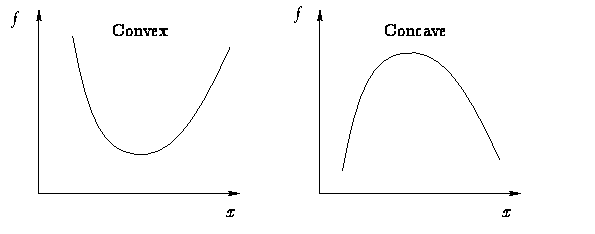
\includegraphics[scale=.5]{convex_concave.png}
  \end{center}
\end{definition}

\begin{definition}{Equivalence Relation}
  A relation is an \textit{Equivalence Relation} if it is
  \begin{enumerate}
    \item Reflexive: $i\leftrightarrow i$.
    \item Symmetric: If $i\to j$ then $j\to i$ .
    \item Transitive: If $i\to j$ and $j\to k$ then $i\to k$.
  \end{enumerate}
\end{definition}

\begin{definition}{Simple Random Walk}
  A \textit{Simple Random Walk} is a random walk which moves only one step at a time. (i.e. $X_{t+1}=X_t\pm1$). A probability $p$ is defined for $\prob(X_{t+1}=X_t+1)$, this means $1-p$ is the probability of stepping in the other direction. A \textit{Simple Random Walk} is \textit{Assymetric} if $p\neq p-1$.
\end{definition}

\subsection{Notation}
\begin{tabular}{|c|c|}
  $p_{x,y}$&$\prob(X_{t+1}=x|X_{t}=y)$ for a \textit{time homogenous markov process}
\end{tabular}

\end{document}
